% no answer key
% \documentclass[letterpaper]{exam}

% answer key
\documentclass[letterpaper, landscape]{exam}
\usepackage{2in1, lscape} 
\printanswers{}

% for the cent symbol
\usepackage{textcomp}

% the textcent command eats the space following the symbol
\usepackage{xspace}
\newcommand{\cent}{\textcent\xspace}

\usepackage{units} 
\usepackage{xfrac} 
\usepackage[fleqn]{amsmath}
\usepackage{cancel}
\usepackage{float}
% \usepackage{mdwlist}
\usepackage{enumitem}
\usepackage{booktabs}
\usepackage{cancel}
\usepackage{polynom}
\usepackage{caption}
\usepackage{fullpage}
\usepackage{comment}
% \usepackage{enumerate}
\usepackage{graphicx}
\usepackage{parskip}

\everymath{\displaystyle}

\title{Statistics \\ Chapter 17 Homework}
\date{\today}
\author{}

\begin{document}

  \maketitle

  \section{Homework}
  Chapter 17: 25--28, 30--31, 33, 35, 38, 44--45, 47

  \ifprintanswers{}
    \section{Solutions}
    \begin{description}

      \item[25] 
        The correct t-statistics and P-values are:
        \begin{itemize}[nosep, label={}]
          \item $t_1 = 0.7490$, $0.4 < P < 0.5$
          \item $t_2 = 3.2769$, $0.005 < P < 0.01 $
        \end{itemize}

        In the first case there isn't a significant difference and in the second case
        there is.

      \item[26] $\mu = 26.8 \pm 0.5756$; $26.2244 < \mu < 27.3756$.

      \item[27]
        \begin{enumerate}[label = (\alph*)]
          \item With a large sample size and limited range data, the normality
            of the population shouldn't be a problem.

          \item $240 \pm 2.8381$ or 237.16 to 242.84

          \item 
            The hypotheses are:
            \begin{itemize}[parsep=0pt,label={}]
              \item $H_0$: $\mu = 243$
              \item $H_a$: $\mu < 243$
            \end{itemize}
            
            This gives $t = -2.7273$ and $0.0025 < P < 0.005$

            With $P < 0.005$, there is strong evidence that the students are below
            average.

        \end{enumerate}

      \item[28]
        \begin{enumerate}[label = (\alph*)]
          \item $\mu = 114.9 \pm 3.6798$; $111.22 < \mu < 118.58$

          \item
            The requirements might include:
            \begin{itemize}
              \item The original 54 subjects are randomly selected from the
                white male population.

              \item The study is only advertised as representing white males.

              \item The subjects were randomly selected for the treatment and
                control groups.

              \item Blood pressure has an approximately Normal distribution.
            \end{itemize}

        \end{enumerate}

      \item[30]
        \begin{figure}[H]
          \centering
          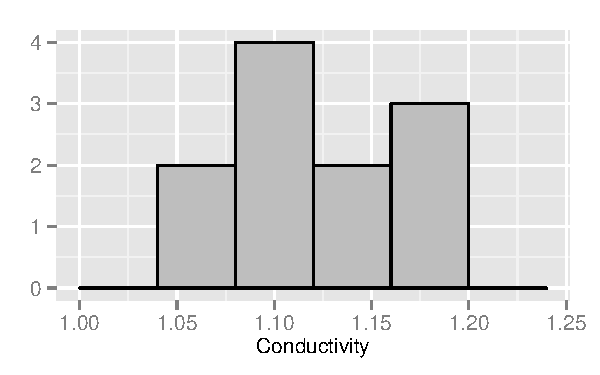
\includegraphics[scale = 1.0]{figures/ex30.pdf}
          \caption{Exercise 30}\label{fig:ex30}
        \end{figure}
        
        \begin{enumerate}[label = (\alph*)]
          \item See Figure~\ref{fig:ex30}. There aren't very many samples, but
            they look evenly distributed.

          \item From the sample: $\bar{x} \approx 1.12$ and $sd \approx 0.044$

            The 95\% confidence interval is:
            
            $\mu = 1.1182 \pm 0.0294$; $1.0888 < \mu < 1.1476$

          \item 
            \begin{itemize}[parsep=0pt,label={}]
              \item $H_0$: $\mu = 1$
              \item $H_a$: $\mu \ne 1$
            \end{itemize}

            With these values, $t = 8.9538$ and $P < 0.001$. There is strong
            evidence that the mean conductivity of the glass is not 1.

        \end{enumerate}

      \item[31]
        \begin{figure}[H]
          \centering
          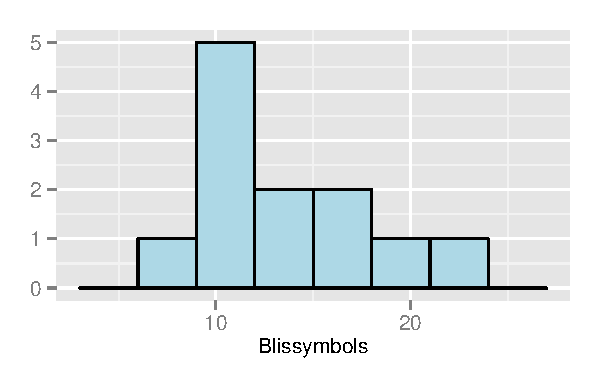
\includegraphics[scale = 1.0]{figures/ex31.pdf}
          \caption{Exercise 31}\label{fig:ex31}
        \end{figure}
        
        \begin{enumerate}[label = (\alph*)]
          \item See Figure~\ref{fig:ex31}. There aren't very many samples, but
            they look fairly Normal.

          \item From the sample: $\bar{x} \approx 12.83$ and $s \approx 4.65$.

            The 90\% confidence interval is: 
            
            $\mu = 12.83 \pm 2.41$; $10.42 < \mu < 15.24$

        \end{enumerate}

      \item[33]
        \begin{figure}[H]
          \centering
          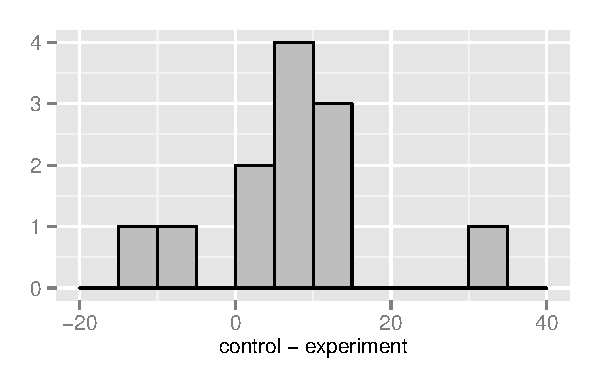
\includegraphics[scale = 1.0]{figures/ex33.pdf}
          \caption{Exercise 33}\label{fig:ex33}
        \end{figure}

        \begin{enumerate}[label = (\alph*)]
          \item See Figure~\ref{fig:ex33}.

          \item 
            With the outlier, there is a significant difference. Without the
            outlier, there (barely) isn't a significant difference.

            \begin{tabular}[H]{lrr}
              \toprule
                              & t      & P-value \\
              \midrule
              with outlier    & 2.0761 & $0.025 < P < 0.05$ \\
              without outlier & 1.7881 & $0.05 < P < 0.1$ \\
              \bottomrule
            \end{tabular}

        \end{enumerate}

      \item[35]
        \begin{figure}[H]
          \centering
          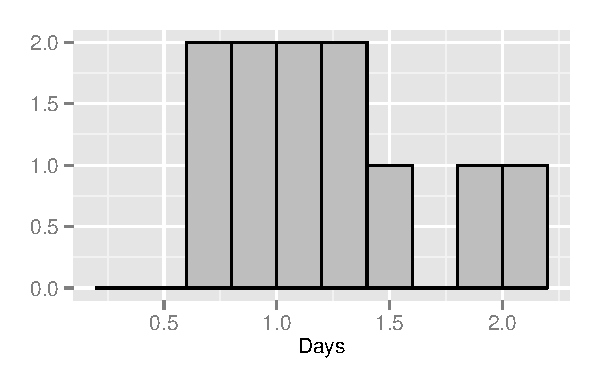
\includegraphics[scale = 1.0]{figures/ex35.pdf}
          \caption{Exercise 35}\label{fig:ex35}
        \end{figure}

        \begin{enumerate}[label = (\alph*)]
          \item See Figure~\ref{fig:ex35}. 
          \item 90\% confidence interval: 
            
            $\mu = 1.1727 \pm 0.2516$; $0.9211 < \mu < 1.4243$ 

            The treatment seems to be effective for these types of patients.

        \end{enumerate}

      \item[38]
        \begin{enumerate}[label = (\alph*)]
          \item The spore count varies quite a bit by day. We want to make sure
            we compare the two rooms on the same day, so that the experiment
            isn't measuring differences between days instead of the difference
            between the two rooms.

          \item $\mu = 1824 \pm 981$; $843 < \mu < 2806$

          \item The sample size is very small. We can be confident that there
            are more spores in the kill room, but not very precise about how
            many more spores there are on average.

        \end{enumerate}

      \item[44]
        \begin{figure}[H]
          \centering
          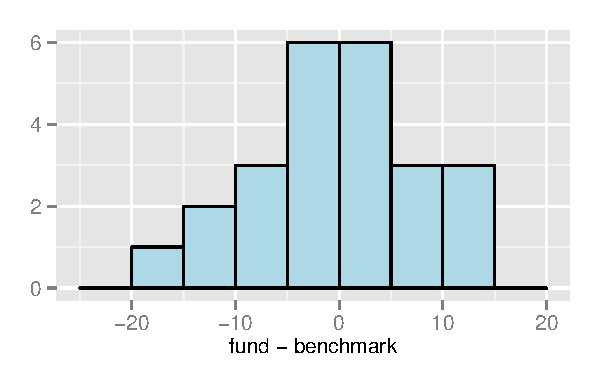
\includegraphics[scale = 1.0]{figures/ex44.pdf}
          \caption{Exercise 44}\label{fig:ex44}
        \end{figure}

        The data look fairly Normal. See Figure~\ref{fig:ex44}.

        The 95\% confidence interval for the mean difference is $-3.45 < \mu < 3.30$.
        Since this interval contains 0, it doesn't rule out the fund exactly matching
        its benchmark.

        The null hypothesis is that the mean difference is 0 and the alternative
        hypothesis is that the mean difference is non-zero.

        $t = -0.0462$ which gives a P-value of 0.9636. This doesn't rule out the
        null hypothesis, so there's no reason to think the fund's performance is
        different from its benchmark.
        
      \item[45]
        \begin{figure}[H]
          \centering
          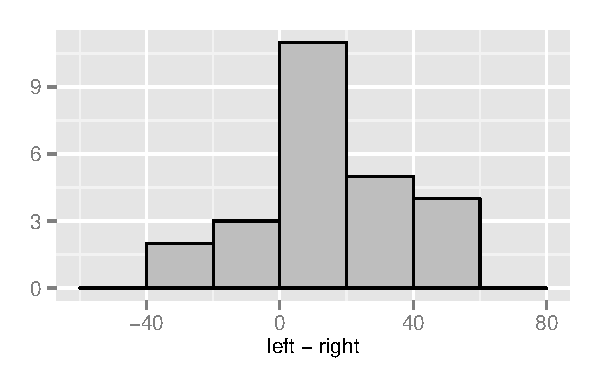
\includegraphics[scale = 1.0]{figures/ex45.pdf}
          \caption{Exercise 45}\label{fig:ex45}
        \end{figure}

        The data look fairly Normal. See Figure~\ref{fig:ex45}.

        The null hypothesis is that the mean difference is 0 and the alternative
        hypothesis is that the mean difference is greater than zero. We should
        use a one-sided t-test.

        t = 2.9037 which gives a one-sided P-value of $0.0025 < P < 0.005$. There is
        a statistically significant difference, $P < 0.005$.
        
      \item[47]

        {\em Approach 1\/}

        \begin{itemize}[parsep=0pt, label={}]
          \item $\bar{x}_{right} = \unit[104.12]{s}$
          \item $\bar{x}_{left} = \unit[117.44]{s}$
        \end{itemize}

        The right hand threads only take 89\% of the time of the left hand
        threads.

        {\em Approach 2\/}

        The 90\% confidence interval for the mean difference is:

        $\unit[5.47]{s} < \mu < \unit[21.17]{s}$.

        It looks like the task takes around 2 minutes, so a worker could do
        about 30 tasks per hour working steadily. 

        If a worker worked 40 hours per week and spent half his time on this
        kind of task, he would do approximately $20 \cdot 30 \approx 600$ tasks
        per week. 
        
        If a worker typically worked 50 weeks per year, he would do about $600
        \cdot 50 = 30,000$ tasks per year.

        If we save 5 to 21 seconds per task, we could save 40 to 175 hours per
        worker per year. 

        This means we could give everybody an extra 1 to 4 weeks of vacation a
        year and still make the same amount of stuff.

  \end{description}

  \else
    \vspace{12 cm}
    \begin{quote}
      \begin{em}
        If the world were perfect, it wouldn't be.
      \end{em}
    \end{quote}
    \hspace{1 cm}--Yogi Berra
  \fi

\end{document}

